
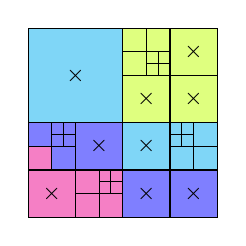
\begin{tikzpicture}[scale=0.6]

  \draw[fill = magenta, fill opacity=0.5] (0,0) rectangle +(1,1);
  \draw (0.5, 0.5) node {\footnotesize{$\times$}};  
  \draw[fill = magenta, fill opacity=0.5] (1,0) rectangle +(0.5, 0.5);  
  \draw[fill = magenta, fill opacity=0.5] (1.5,0) rectangle +(0.5,0.5);  
  \draw[fill = magenta, fill opacity=0.5] (1,0.5) rectangle +(0.5,0.5);
  \draw[fill = magenta, fill opacity=0.5] (1.5,0.5) rectangle +(0.25,0.25);  
  \draw[fill = magenta, fill opacity=0.5] (1.75,0.5) rectangle +(0.25,0.25);
  \draw[fill = magenta, fill opacity=0.5] (1.5,0.75) rectangle +(0.25,0.25);
  \draw[fill = magenta, fill opacity=0.5] (1.75,0.75) rectangle +(0.25,0.25);
  \draw[fill = magenta, fill opacity=0.5] (0,1) rectangle +(0.5,0.5);
  
  \draw[fill = blue, fill opacity=0.5] (0.5,1) rectangle +(0.5,0.5);
  \draw[fill = blue, fill opacity=0.5] (0,1.5) rectangle +(0.5,0.5);
  \draw[fill = blue, fill opacity=0.5] (0.5,1.5) rectangle +(0.25,0.25);
  \draw[fill = blue, fill opacity=0.5] (0.75,1.5) rectangle +(0.25,0.25);
  \draw[fill = blue, fill opacity=0.5] (0.5,1.75) rectangle +(0.25,0.25);
  \draw[fill = blue, fill opacity=0.5] (0.75,1.75) rectangle +(0.25,0.25);
  \draw[fill = blue, fill opacity=0.5] (1,1) rectangle +(1,1);  
  \draw (1.5, 1.5) node {\footnotesize{$\times$}};
  \draw[fill = blue, fill opacity=0.5] (2,0) rectangle +(1,1);
  \draw (2.5, 0.5) node {\footnotesize{$\times$}};
  \draw[fill = blue, fill opacity=0.5] (3,0) rectangle +(1,1);
  \draw (3.5, 0.5) node {\footnotesize{$\times$}};
  
  \draw[fill = cyan, fill opacity=0.5] (2,1) rectangle +(1,1);
  \draw (2.5, 1.5) node {\footnotesize{$\times$}};
  \draw[fill = cyan, fill opacity=0.5] (3,1) rectangle +(0.5,0.5);
  \draw[fill = cyan, fill opacity=0.5] (3.5,1) rectangle +(0.5,0.5);
  \draw[fill = cyan, fill opacity=0.5] (3,1.5) rectangle +(0.25,0.25);
  \draw[fill = cyan, fill opacity=0.5] (3.25,1.5) rectangle +(0.25,0.25);
  \draw[fill = cyan, fill opacity=0.5] (3,1.75) rectangle +(0.25,0.25);
  \draw[fill = cyan, fill opacity=0.5] (3.25,1.75) rectangle +(0.25,0.25);
  \draw[fill = cyan, fill opacity=0.5] (3.5,1.5) rectangle +(0.5,0.5);    
  \draw[fill = cyan, fill opacity=0.5] (0,2) rectangle +(2,2);
  \draw (1, 3) node {\footnotesize{$\times$}};
  
  \draw[fill = lime, fill opacity=0.5] (2,2) rectangle +(1,1);
  \draw (2.5, 2.5) node {\footnotesize{$\times$}};
  \draw[fill = lime, fill opacity=0.5] (3,2) rectangle +(1,1);
  \draw (3.5, 2.5) node {\footnotesize{$\times$}};
  \draw[fill = lime, fill opacity=0.5] (2,3) rectangle +(0.5,0.5);
  \draw[fill = lime, fill opacity=0.5] (2.5,3) rectangle +(0.25,0.25);
  \draw[fill = lime, fill opacity=0.5] (2.75,3) rectangle +(0.25,0.25);
  \draw[fill = lime, fill opacity=0.5] (2.5,3.25) rectangle +(0.25,0.25);
  \draw[fill = lime, fill opacity=0.5] (2.75,3.25) rectangle +(0.25,0.25);
  \draw[fill = lime, fill opacity=0.5] (2,3.5) rectangle +(0.5,0.5);
  \draw[fill = lime, fill opacity=0.5] (2.5,3.5) rectangle +(0.5,0.5);
  \draw[fill = lime, fill opacity=0.5] (3,3) rectangle +(1,1);
	\draw (3.5, 3.5) node {\footnotesize{$\times$}};
	  		
\end{tikzpicture}  